\subsection{Architecture}
In het begin van de archtectuur definieren we de benodigde signalen. Op basis van cnt en pwmi kunnen we gemakkelijk een PWM singaal laten generen (verder meer details over hoe). Daarna worden de nodige types en signalen aangemaakt om een statenmachine te kunnen gebruiken. Eerst worden de verschillende staten gedefinieerd waarna de signalen voor het bijhouden van de staat ook aangemaakt worden.

\lstinputlisting[firstline=1,lastline=14]{servocontroller_arch.vhd}
state\_trans beschrijft de transities tussen verschillende staten. Hierbij hoort volgende flowchart.
\begin{figure}[h]
	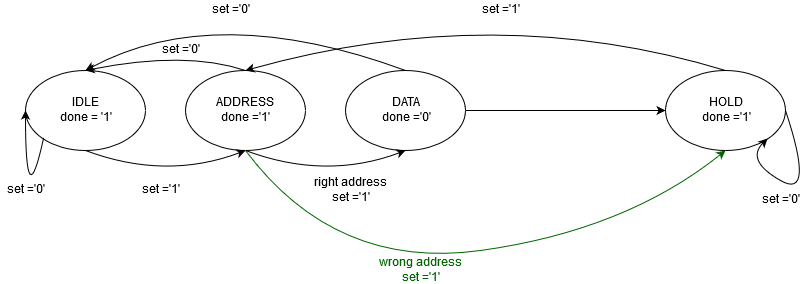
\includegraphics[width=\linewidth]{servocontrol.png}
\end{figure}\\
Hierbij moet rekening gehouden worden met een aantal dingen. Zo is er een reset met hoogste prioriteit, deze heeft altijd voorrang. Moet er gekeken worden of het address juist is of het address het broadcast address is. Indien de set onderbroken wordt, moet de controller naar de neutrale positie gaan.

\lstinputlisting[firstline=16,lastline=52]{servocontroller_arch.vhd}
transition is gewoon het synchroon proces dat de overgangen van de staten dicteert.

\lstinputlisting[firstline=54,lastline=59]{servocontroller_arch.vhd}
set\_output dicteert hoe de output signalen zich gedragen in elke staat. In deze setup stelt zich dit zo dat Done een 3 state logic heeft. Het PWM signaal wordt hier niet gedfinieerd omdat er een oneliner gebruikt wordt om dit aan de uitgang te koppelen (zie verder).

\lstinputlisting[firstline=61,lastline=80]{servocontroller_arch.vhd}
pwm\_data is het proces dat de berekeningen en lengte van de puls bepaalt. Op basis van de servoklok wordt berekend welke waarden nodig zijn om de gewenste pulsen te bekomen. In de commentaar zijn de berekende waarden voor een servoklok van 510kHz te vinden. Indien de servoklok aangepast wordt, met deze code aangepast worden zodat de juiste waarden gebruikt worden.

\lstinputlisting[firstline=82,lastline=98]{servocontroller_arch.vhd}
gen\_pwm is het proces dat de eigenlijk puls genereert. Het aantal servoklok ticks wordt bijgehouden en vergelijken met de benodigde aantallen die is pwm\_data bepaald zijn. cnt moet gerest wordne bij elke klok tick.\\
Nadien wordt met een oneliner eigenlijk het pwm signaal gegenereert door een klein procesje dat reageert op de veranderingen in gen\_pwm.

\lstinputlisting[firstline=100,lastline=113]{servocontroller_arch.vhd}